\date{}
\title{}
\date{}
\usepackage{pdfpages}
\begin{document}
\begin{frame}
    \titlepage
\end{frame}


\makeatletter
\newenvironment<>{btHighlight}[1][]
{\begin{onlyenv}#2\begingroup\tikzset{bt@Highlight@par/.style={#1}}\begin{lrbox}{\@tempboxa}}
{\end{lrbox}\bt@HL@box[bt@Highlight@par]{\@tempboxa}\endgroup\end{onlyenv}}

\newcommand<>\btHL[1][]{%
  \only#2{\begin{btHighlight}[#1]\bgroup\aftergroup\bt@HL@endenv}%
}
\def\bt@HL@endenv{%
  \end{btHighlight}%   
  \egroup %
}
\tikzset{
    btHLbox/.style={
        fill=red!30,outer sep=0pt,inner xsep=1pt, inner ysep=0pt, rounded corners=3pt
    },
}
\newcommand{\bt@HL@box}[2][]{%
  \tikz[#1]{%
    \pgfpathrectangle{\pgfpoint{1pt}{0pt}}{\pgfpoint{\wd #2}{\ht #2}}%
    \pgfusepath{use as bounding box}%
    \node[text width={},draw=none,anchor=base west, btHLbox, minimum height=\ht\strutbox+1pt,#1]{\raisebox{1pt}{\strut}\strut\usebox{#2}};
  }%
}

\lst@CCPutMacro
    \lst@ProcessOther {"2A}{%
      \lst@ttfamily 
         {\raisebox{2pt}{*}}% used with ttfamily
         {\raisebox{2pt}{*}}}% used with other fonts
    \@empty\z@\@empty

\lstdefinelanguage
   [x8664gas]{Assembler}     % add a "x64" dialect of Assembler
   [x86masm]{Assembler} % based on the "x86masm" dialect
   % with these extra keywords:
   {morekeywords={CDQE,CQO,CMPSQ,CMPXCHG16B,JRCXZ,LODSQ,MOVSXD,%
                  POPFQ,PUSHFQ,SCASQ,STOSQ,IRETQ,RDTSCP,SWAPGS,.TEXT,.STRING,.ASCIZ,%
                  BEQ,LW,SW,LB,SB,ADDIU,J,BEQZ,BNEZ,BNE,%
                  MOVUPD,MULPD,MOVSD,MULSD,%
                  SHLADD,MOV,CMP.LT,TBIT.NZ,BR.RET.SPTK.MANY,%
                  ADDQ,POPQ,PUSHQ,RRMOVQ,MRMOVQ,RMMOVQ,IRMOVQ,%
                  <-,LL,SC,ADDI,ADDL,VMOVDQA,ADDQ,CMPL,JB,JBE,MOVL,CLTQ,
                  MOVW,PUSHW,MOV,ADD,SUB,INT,PUSH,MOV,ADD,REP,MOVSB,%
                  TESTQ,CMPQ,MOVL,MOVQ,ADDQ,JMPQ,XORQ,%
                  LEAQ,LEAL,LEA,RETQ,RET,POPL,POPW,PUSHL,PUSHW,%
                  LEAW,%
                  SUBQ,SYSCALL,.ASCII,CALLQ,MOVSLQ,JMP,ANDQ,SHRQ,MOVB,INCQ,TESTL,XORL,%
                  SHRL,LEAL,SARL,SUBL,IMULL,IMULQ,MOVDQU,PADDD,XORL,%
                  MOVZBL,MOVZB,SHRB,SRAL,SHRL,ANDL,%
                  CMOVNS,SRAL,SRAQ,MOVZBW,MOVZBQ,%
                  PADDW,PADDQ,MODUPS,MOVAPD,%
                  MOVL,RET,.GLOBL,%
                  },
    deletekeywords={eax,ebx,sp,si,cx,di,ds,cs,es,fs,dx,ax,bx,al,esi,ebp,ecx,rip,eip,edx,edi,rdi,esp},
    morecomment=[l]{\#},
    morecomment=[l]{\/\/},
    morecomment=[s]{/*}{*/},
    sensitive=false,
    keepspaces=true} % et

\lstalias[]{myasm}[x8664gas]{Assembler}

\lstdefinelanguage{JavaScript}{
  keywords={typeof, new, true, false, catch, function, return, null, catch, switch, var, if, in, while, do, else, case, break},
  ndkeywords={class, export, boolean, throw, implements, import, this},
  sensitive=false,
  comment=[l]{//},
  morecomment=[s]{/*}{*/},
  morestring=[b]',
  morestring=[b]"
}

\newcommand{\keywordstyle}{\sourcecodeprolight\bfseries\color{blue!30!black}}
\newcommand{\stringstyle}{\color{blue!20!black}\ttfamily}

\lstset{
    language=C,
    basicstyle=\sourcecodepro\EmptyMapping,
    escapechar=`,
    keywordstyle=\keywordstyle\EmptyMapping,
    identifierstyle=\sourcecodepro\EmptyMapping,
    numberstyle=\small\color{black!70},
    commentstyle=\color{red!60!black}\ttfamily\itshape,
    stringstyle=\color{blue!20!black}\ttfamily,
    ndkeywordstyle=\bfseries\color{blue!30!black},
    upquote=true,
}



\lstdefinestyle{medium}{
    basicstyle=\sourcecodepro\EmptyMapping\fontsize{12}{13}\selectfont,
    keywordstyle=\sourcecodepro\EmptyMapping\fontsize{12}{13}\selectfont\keywordstyle,
}

\lstdefinestyle{small}{
    basicstyle=\sourcecodepro\EmptyMapping\small,
    keywordstyle=\sourcecodepro\EmptyMapping\small\keywordstyle,
}

\lstdefinestyle{smaller}{
    basicstyle=\sourcecodepro\EmptyMapping\fontsize{11}{12}\selectfont,
    keywordstyle=\sourcecodepro\EmptyMapping\fontsize{11}{12}\selectfont\keywordstyle,
}


\lstdefinestyle{script}{
    basicstyle=\sourcecodepro\EmptyMapping\scriptsize,
    keywordstyle=\sourcecodepro\EmptyMapping\scriptsize\bfseries,
}



\section{last time}
\begin{frame}{last time (1)}
    \begin{itemize}
    \item side channel idea:
        \begin{itemize}
        \item unintended information leakage
        \item example: time taken to check password $\rightarrow$ matching character count
        \end{itemize}
    \item in the cache: PRIME+PROBE strategy
        \begin{itemize}
        \item timing difference indicates what's in cache
        \item evictions reveal index bits of cache accesses
        \end{itemize}
    \item speculative execution and cache accesses
        \begin{itemize}
        \item OOO processors still run cache accesses on branch misprediction
        \item problem: branches do things like bounds check
        \item way of reading out-of-bounds data
        \end{itemize}
    \end{itemize}
\end{frame}

\begin{frame}[fragile]{last time (2)}
    \begin{itemize}
    \item Meltdown 
        \begin{itemize}
        \item some Intel CPUs: speculative page table permissions check
        \item \verb|if (false) { access array[*kernel_memory * factor] }|
        \item idea: array access adds to cache (even though undone)
        \item detect what was evicted, learn \verb|*kernel_memory| value
        \end{itemize}
    \item Spectre
        \begin{itemize}
        \item \verb|if (x < size) { access array2[array1[x] * factor] }|
        \item if statement mispredicted, so array2 access modifies cache
        \item \ldots can detect which cache index accessed
        \item pattern appears naturally in system calls, etc.
        \item learn \verb|array1[x]| value, even though out of bounds
        \end{itemize}
    \end{itemize}
\end{frame}

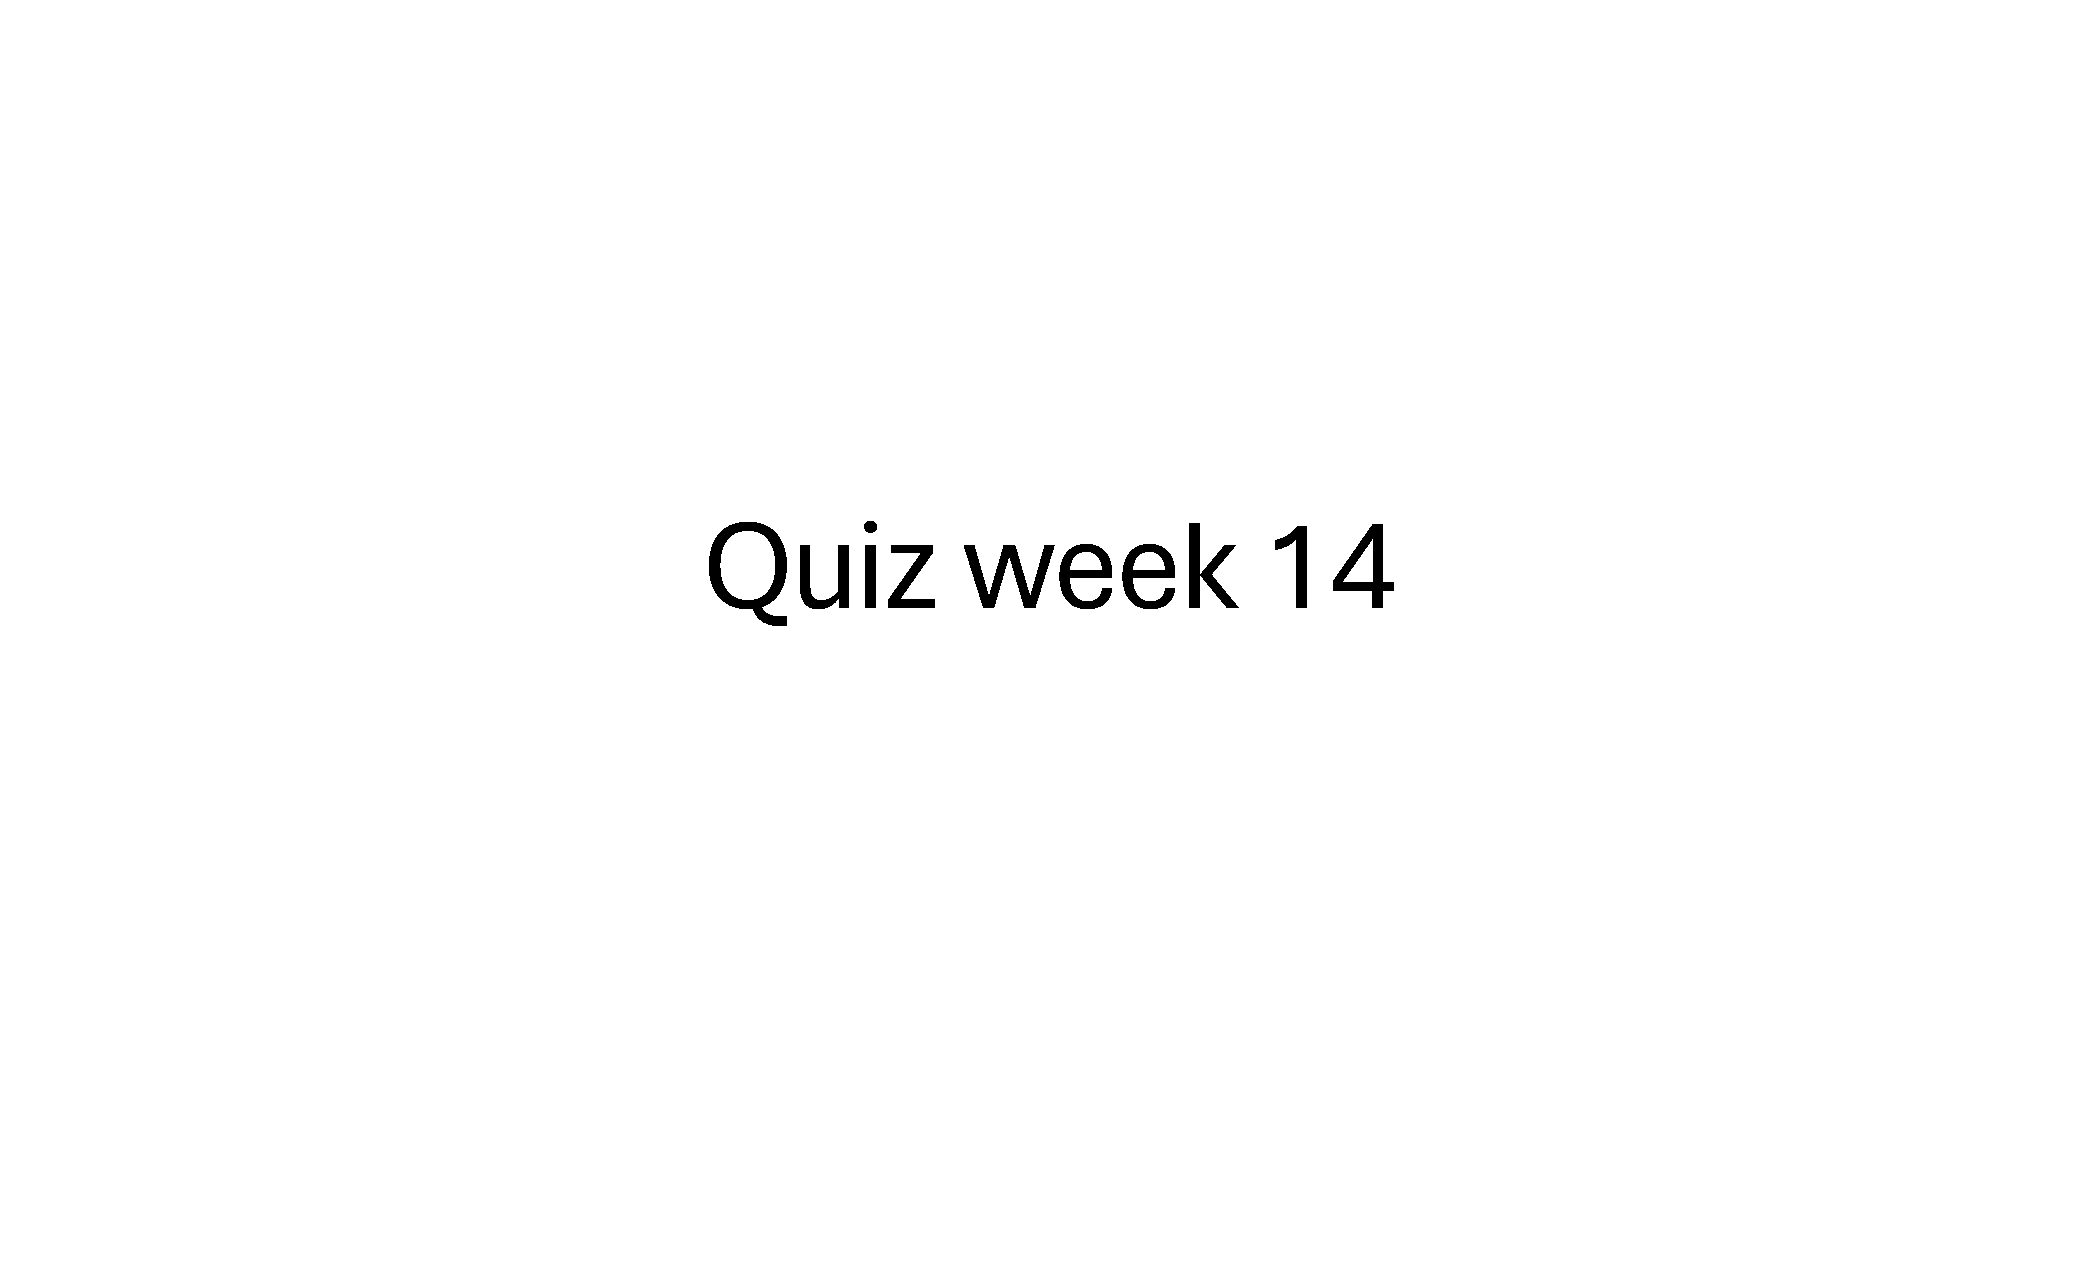
\includepdf[pages=1-]{3130_Dec3_quiz14}

\includepdf[pages=1-]{3130_Dec3_spectre2}

\section{spectre}

\begin{frame}[fragile]{review: PRIME+PROBE}
\begin{Verbatim}[fontsize=\small]
char *array;
// PRIME
posix_memalign(&array, CACHE_SIZE, CACHE_SIZE);
AccessAllOf(array);

// (some code we don't control)
other_array[mystery * BLOCK_SIZE] += 1;

// PROBE
for (int i = 0; i < CACHE_SIZE; i += BLOCK_SIZE) {
    if (CheckIfSlowToAccess(&array[i])) {
    ...
    }
}
\end{Verbatim}
\end{frame}


\begin{frame}[fragile]{exercise}
\begin{Verbatim}[fontsize=\fontsize{9}{10}]
char *array;
// PRIME
posix_memalign(&array, CACHE_SIZE, CACHE_SIZE);
AccessAllOf(array);
// (some code we don't control)
other_array[mystery * BLOCK_SIZE] += 1;
// PROBE
for (int i = 0; i < CACHE_SIZE; i += BLOCK_SIZE) {
    if (CheckIfSlowToAccess(&array[i])) {
    ...
    }
}
\end{Verbatim}
\begin{itemize}
\item 64KB ($2^{16}$B) direct-mapped cache with 64B blocks
\item array[0x800] slow to access; \item other\_array at \texttt{0x4000000}
\item value of \texttt{mystery}?
\end{itemize}
\end{frame}

\begin{frame}[fragile]{exercise solution (1)}
\begin{itemize}
\item NUM\_SETS = 64KB/64B = 1K (1024) sets
\item array[0x800] has cache index {\small \texttt{0x800}/BLOCK\_SIZE mod NUM\_SETS}
    \begin{itemize}
    \item = cache index 32
    \end{itemize}
\item know \texttt{\small other\_array[mystery * BLOCK\_SIZE]} had same index
\vspace{.5cm}
\item \texttt{other\_array[0]} at cache index 0
    \begin{itemize}
    \item (0x4000000 / BLOCK\_SIZE) mod NUM\_SETS = 0
    \end{itemize}
\end{itemize}
\end{frame}

\begin{frame}[fragile]{exercise solution (2)}
\begin{itemize}
\item recall have found:
    \begin{itemize}
    \item \texttt{other\_array[0]} at index 0;
    \item \texttt{other\_array[mystery*BLOCK\_SIZE]} has index 32 (same as \texttt{array[0x800]})
    \end{itemize}
\item \texttt{other\_array[X]} at cache index (0 + X/BLOCK\_SIZE  mod NUM\_SETS)
    \begin{itemize}
    \item advanced by X/BLOCK\_SIZE blocks
    \item wrapping around after NUM\_SETS blocks
    \end{itemize}
\vspace{.5cm}
\item X = mystery * BLOCK\_SIZE
\item 32 = 0 + mystery mod NUM\_SETS
\item mystery = 32 or 32 $\pm$ 1024 or 32 $\pm$ 1024 $\times$ 2 or etc.
\end{itemize}
\end{frame}



\begin{frame}{variation: different starting location}
    \begin{itemize}
    \item other\_array starts at 0x4001440
    \item then other\_array[0] at cache index 
        \begin{itemize}
        \item 0x4001440 / BLOCK\_SIZE mod NUM\_SETS = 51
        \end{itemize}
    \item (51 + mystery * BLOCK\_SIZE / BLOCK\_SIZE) mod NUM\_SETS = 32
    \item mystery = -19 or 1005 or 2029 or \ldots
    \end{itemize}
\end{frame}

\begin{frame}[fragile]{variation: associative cache}
\begin{Verbatim}[fontsize=\fontsize{9}{10}]
char *array;
// PRIME
posix_memalign(&array, CACHE_SIZE, CACHE_SIZE);
AccessAllOf(array);
// (some code we don't control)
other_array[mystery * BLOCK_SIZE] += 1;
// PROBE
for (int i = 0; i < CACHE_SIZE; i += BLOCK_SIZE) {
    if (CheckIfSlowToAccess(&array[i])) { ...  }
}
\end{Verbatim}
    \begin{itemize}
    \item suppose 2-way 64KB cache instead of direct-mapped
    \item NUM\_SETS = 64KB/2/64B = 512 sets
    \item array[0x800] still has cache index 32 (still)
    \item but now mystery can be $32$ or $32+512$ or $32+512\cdot2$ or \ldots
    \end{itemize}
\end{frame}

\begin{frame}[fragile]{variation: associative cache (2)}
\begin{Verbatim}[fontsize=\fontsize{9}{10}]
char *array;
// PRIME
posix_memalign(&array, CACHE_SIZE, CACHE_SIZE);
AccessAllOf(array);
// (some code we don't control)
other_array[mystery * BLOCK_SIZE] += 1;
// PROBE
for (int i = 0; i < CACHE_SIZE; i += BLOCK_SIZE) {
    if (CheckIfSlowToAccess(&array[i])) { ...  }
}
\end{Verbatim}
    \begin{itemize}
    \item suppose 2-way 64KB cache w/ 64B and \myemph{\tt array[0x8800]} is slow
    \item 0x8800/BLOCK\_SIZE = 544 = 512 + 32
    \item since 512 sets total, still set index 32
    \item mystery still $32$ or $32+512$ or $32+512\cdot2$ or \ldots
    \end{itemize}
\end{frame}

\begin{frame}{exercise}
\begin{itemize}
\item if 4-way 64KB cache w/64B blocks and something from cache set 32 evicted,\\
then where could slow access be?
    \begin{itemize}
    \item recall: 2-way cache: i=0x800, i=0x8800
    \end{itemize}
\item A. i=0x400, i=0x800, i=0x8400, i=0x8800
\item B. i=0x800, i=0x8800, i=0x10800, i=0x18800
\item C. i=0x800, i=0x4800, i=0x8800, i=0xc800
\item D. i=0x800, i=0x4800, i=0x8800, i=0x10800
\item E. something else
\end{itemize}
\end{frame}


\begin{frame}[fragile]{not just BLOCK\_SIZE}
\begin{Verbatim}[fontsize=\fontsize{9}{10}]
char *array;
// PRIME
posix_memalign(&array, CACHE_SIZE, CACHE_SIZE);
AccessAllOf(array);
// (some code we don't control)
other_array[mystery * N] += 1;  // previously: * BLOCK_SIZE
// PROBE
for (int i = 0; i < CACHE_SIZE; i += BLOCK_SIZE) {
    if (CheckIfSlowToAccess(&array[i])) {
    ...
    }
}
\end{Verbatim}
\begin{itemize}
\item 64KB ($2^{16}$B) direct-mapped cache with 64B blocks
\item array[0x800] slow to access?
\item other\_array at \texttt{0x4000000} (index 0, offset 0)
\item value of \texttt{mystery} if N = 1? N = 32 * 64?
\end{itemize}
\end{frame}

\begin{frame}{solution (N=1)}
\vspace{-1cm}
\begin{eqnarray*}
\left\lfloor\text{mystery} * N / \text{BLOCK\_SIZE}\right\rfloor~\text{mod}~1024 & = & 32 \\
\left\lfloor\text{mystery} * N / \text{BLOCK\_SIZE}\right\rfloor & = & 32 + 1024K \\
\end{eqnarray*}
\\
let offset be some number in [0,BLOCK\_SIZE): \\
\vspace{-1cm}
\begin{eqnarray*}
\text{mystery} * N & = & \text{BLOCK\_SIZE}\times(32+1024K) + \text{offset}\\
\text{mystery} & = & \text{BLOCK\_SIZE}\times(32+1024K) + N\times\text{offset} \\
\text{mystery} & = & 64\times(32+1024K)+N\times\text{offset} \\
\end{eqnarray*}
\\
N=1: mystery = $2048$, $2049$, $2050$, \ldots, $2048+63$, $64\cdot1024+2048$, $64\cdot1024+2048+1$, \ldots
\end{frame}

\begin{frame}{exercise (N=32*64)}
    \begin{itemize}
    \item what if N = 32*64
    \item recall: other\_array[0] is set 0, offset 0
    \item other\_array[mystery * N] is set 32
    \item possible values of mystery?
    \end{itemize}
\vspace{-.5cm}
\begin{eqnarray*}
\text{mystery}\cdot 32\cdot 64 & = & 64(32+1024K) + \text{offset} \\
        & = & 64\cdot32 + 65536K + \text{offset}\\
\text{mystery} & = & 1 + \frac{65536}{64\cdot32}K + \frac{\text{offset}}{64\cdot32} = 1+32K \\
\end{eqnarray*}
\end{frame}

\begin{frame}{alternate view}
    \begin{itemize}
    \item learn index bits of mystery * N
    \item this example: bits 6--15
    \vspace{.5cm}
    \item N = 1, bits 6--15 of mystery
    \item N = 64, bits 0--9 of mystery
    \item N = 32*64 ($2^{11}$), bits 0--4 of mystery
    \end{itemize}
\end{frame}


\providecommand{\myemphA}[1]{\myemph<2>{#1}}
\providecommand{\myemphB}[1]{\myemph<3>{#1}}

\begin{frame}[fragile]{EVICT+RELOAD}
    \begin{itemize}
    \item PRIME+PROBE: fill cache, detect eviction
    \item alternate idea \myemph<2>{EVICT}+\myemph<3>{RELOAD}:
    \end{itemize}
\begin{Verbatim}[fontsize=\small,commandchars=\\QX]
unsigned char *probe_array;
posix_memalign(&probe_array, CACHE_SIZE, CACHE_SIZE);
\myemphAQaccess OTHER things to evict all of probe_arrayX
if (something false) {
    read probe_array[mystery * BLOCK_SIZE];
}
\myemphBQcheck which value from probe_array is fasterX
\end{Verbatim}
\begin{itemize}
\item requires code to access something you can access
\item but often easier to setup/more reliable than PRIME+PROBE
\end{itemize}
\end{frame}



% FIXME to Skad: mention that this is Meltdown
% FIXME to Skad: alternate to PRIME+PROBE: EVICT+RELOAD
\begin{frame}[fragile]{into exploit: Meltdown}
\begin{Verbatim}[fontsize=\small]
uint8_t* probe_array = new uint8_t[256 * 4096];
// ... Make sure probe_array is not cached
uint8_t kernel_memory_val = *(uint8_t*)(kernel_address);
uint64_t final_kernel_memory = kernel_memory_val * 4096;
uint8_t dummy = probe_array[final_kernel_memory];
// ... catch page fault
// ... in signal handler, determine which of 256 slots in probe_array is cached
\end{Verbatim}
\end{frame}



\subsection{concept: forcing branch misprediction}
%\againframe<2>{readWithoutRead}
\begin{frame}[fragile]{mistraining branch predictor?}
\begin{lstlisting}[language=C]
if (something) {
    CodeToRunSpeculatively()
}
\end{lstlisting}
\begin{itemize}
\item how can we have `something' be false, but predicted
    as true
\vspace{.5cm}
\item run lots of times with something true
\item then do actually run with something false
\end{itemize}
\end{frame}



\subsection{contrived? vulnerable code}
\begin{frame}[fragile]{contrived(?) vulnerable code (1)}
\begin{itemize}
\item suppose this C code is run with extra privileges
    \begin{itemize}
    \item (e.g. in system call handler, library called from JavaScript in webpage, etc.)
    \end{itemize}
\item assume \texttt{x} chosen by attacker
\item (example from original Spectre paper)
\end{itemize}
\begin{lstlisting}
if (x < array1_size)
        y = array2[array1[x] * 4096];
\end{lstlisting}
\end{frame}

\begin{frame}[fragile]{the out-of-bounds access (1)}
\begin{lstlisting}
char array1[...];
...
int secret;
...
y = array2[array1[x] * 4096];
\end{lstlisting}
\begin{itemize}
\item suppose array1 is at \texttt{0x1000000} and
\item secret is at \texttt{0x103F0003};
\item what x do we choose to make \lstinline|array1[x]| access first byte of secret?
\end{itemize}
\end{frame}

\begin{frame}[fragile]{the out-of-bounds access (2)}
\begin{lstlisting}
char array1[...];
...
int secret;
...
y = array2[array1[x] * 4096];
\end{lstlisting}
\begin{itemize}
\item suppose our cache has 64-byte blocks and 8192 sets
\item and \lstinline|array2[0]| is stored in cache set 0
\vspace{.5cm}
\item if the above evicts something in cache set 128, \\
      then what do we know about \texttt{array1[x]}?
    \begin{itemize}
    \item<2-> is 2 or 254
    \end{itemize}
\end{itemize}
\end{frame}

\begin{frame}[fragile]{exploit with contrived(?) code}
\begin{lstlisting}[language=C,style=smaller]
/* in kernel: */
int systemCallHandler(int x) {
    if (x < array1_size)
        y = array2[array1[x] * 4096];
    return y;
}
\end{lstlisting}
\hrule
\begin{lstlisting}[language=C,style=smaller]
/* exploiting code */
    /* step 1: mistrain branch predictor */
for (a lot) {
    systemCallHandler(0 /* less than array1_size */);
}
    /* step 2: evict from cache using misprediction */
Prime();
systemCallHandler(targetAddress - array1Address);
int evictedSet = ProbeAndFindEviction();
int targetValue = (evictedSet - array2StartSet) / setsPer4K;
\end{lstlisting}
\end{frame}


\subsection{array bounds check}
\begin{frame}[fragile]{really contrived?}
\begin{lstlisting}[language=C,style=smaller]
char *array1; char *array2;
if (x < array1_size)
    y = array2[array1[x] * 4096];
\end{lstlisting}
\begin{itemize}
\item times 4096 shifts so we can get lower bits of target value
    \begin{itemize}
    \item so all bits effect what cache block is used
    \end{itemize}
\end{itemize}
\hrule
\begin{visibleenv}<2->
\begin{lstlisting}[language=C,style=smaller]
int *array1; int *array2;
if (x < array1_size)
    y = array2[array1[x]];
\end{lstlisting}
\begin{itemize}
\item will still get \textit{upper} bits of array1[x] (can tell from cache set)
\item<2-> can still read arbitrary memory!
    \begin{itemize}
    \item want memory at 0x10000?
    \item upper bits of 4-byte integer at 0x3FFFE
    \end{itemize}
\end{itemize}
\end{visibleenv}
\end{frame}

\begin{frame}[fragile]{bounds check in kernel}
\lstset{
    language=C,
    style=small,
    moredelim={**[is][\btHL<2>]{@2}{2@}},
    moredelim={**[is][\btHL<3>]{@3}{3@}},
    moredelim={**[is][\btHL<4>]{@4}{4@}},
    moredelim={**[is][\btHL<5>]{@5}{5@}},
}
\begin{tikzpicture}
\node[draw,very thick,text width=10cm,label={east:actual code}] (syscall) {
\begin{lstlisting}
void SomeSystemCallHandler(int index) {
    if (@2index > some_table_size2@) 
        return ERROR;
    int kind = @3table[index]3@;
    switch (@4other_table[kind].foo4@) {
        ...
    }
}
\end{lstlisting}
};
\node[draw,very thick,anchor=south west,text width=10cm,label={east:our template}] (template) at (syscall.north west) {
\begin{lstlisting}
if (@2x < array1_size2@) {
    y = @4array2[@3array1[x]3@]4@);
}
\end{lstlisting}
};
\end{tikzpicture}
\end{frame}


\subsection{JavaScript exploit}
\begin{frame}{privilege levels?}
    \begin{itemize}
    \item vulnerable code runs with higher privileges
    \item so far: higher privileges = kernel mode
    \vspace{.5cm}
    \item but other common cases of higher privileges
    \item example: scripts in web browsers
    \end{itemize}
\end{frame}

\begin{frame}[fragile]{JavaScript}
\begin{itemize}
\item JavaScript: scripts in webpages
\item not supposed to be able to read arbitrary memory, but\ldots
\item can access arrays to examine caches
\item and could take advantage of some browser function being vulnerable
\vspace{.5cm}
\item<2-> or --- \myemph<2>{doesn't even need browser to supply vulnerable code itself!}
\end{itemize}
\end{frame}

\begin{frame}[fragile]{just-in-time compilation?}
\begin{itemize}
\item for performance, compiled to machine code, run in browser
\item not supposed to be access arbitrary browser memory
\item example JavaScript code from paper:
\end{itemize}
\begin{lstlisting}[language=JavaScript,style=small]
if (index < simpleByteArray.length) {
    index = simpleByteArray[index | 0];
    index = (((index * 4096)|0) & (32*1024*1024-1))|0;
    localJunk ˆ= probeTable[index|0]|0;
}
\end{lstlisting}
\begin{itemize}
\item web page runs a lot to train branch predictor
\item then does run with out-of-bounds index
\item examines what's evicted by probeTable access
\end{itemize}
\end{frame}


\subsection{mispredicted indirect}
\begin{frame}[fragile]{other misprediction}
\begin{itemize}
\item so far: talking about mispredicting direction of branch
\item what about mispredicting target of branch in, e.g.:
\end{itemize}
\begin{lstlisting}
// possibly from C code like:
//   (*function_pointer)();
jmp *%rax           

// possibly from C code like:
//      switch(rcx) { ... }
jmp *(%rax,%rcx,8)  
\end{lstlisting}
\end{frame}

\begin{frame}[fragile]{an idea for predicting indirect jumps}

for jmps like \lstinline|jmp *%rax| predict target with cache: \\
\begin{tabular}{ll}
bottom 12 bits of jmp address & last seen target \\ \hline
0x0--0x7 & 0x200000 \\
0x8--0xF & 0x440004 \\
0x10-0x18 & 0x4CD894 \\
0x18-0x20 & 0x510194 \\
0x20-0x28 & 0x4FF194 \\
\ldots & \ldots \\
0xFF8--0xFFF & 0x3F8403 \\
\end{tabular}
\begin{itemize}
\item Intel Haswell CPU did something similar to this
    \begin{itemize}
    \item uses bits of last several jumps, not just last one
    \end{itemize}
\item can mistrain this branch predictor
\end{itemize}
\end{frame}

\begin{frame}[fragile]{using mispredicted jump}
\begin{itemize}
\item 1: find some kernel function with \lstinline|jmp *%rax|
\item 2: mistrain branch target predictor for it to jump to chosen code
    \begin{itemize}
    \item use code at address that conflicts in ``recent jumps cache''
    \end{itemize}
\item 3: have chosen code be attack code (e.g. array access)
    \begin{itemize}
    \item either write special code OR
    \item find suitable instructions (e.g. array access) in existing kernel code
    \end{itemize}
\end{itemize}
\end{frame}



\subsection{more variants?}
\begin{frame}{Spectre variants}
    \begin{itemize}
    \item showed Spectre variant 1 (array bounds), 2 (indirect jump)
        \begin{itemize}
        \item from original paper
        \end{itemize}
    \vspace{.5cm}
    \item other possible variations:
        \begin{itemize}
        \item could cause other things to be mispredicted
            \begin{itemize}
            \item prediction of where functions return to?
            \item values instead of which code is executed?
            \end{itemize}
        \item could use side-channel other than data cache changes
            \begin{itemize}
            \item instruction cache
            \item cache of pending stores not yet committed
            \item contention for resources on multi-threaded CPU core
            \item branch prediction changes
            \item \ldots
            \end{itemize}
        \end{itemize}
    \end{itemize}
\end{frame}


\subsection{software fix}
\begin{frame}[fragile]{some Linux kernel mitigations (1)}
\begin{itemize}
\item replace \lstinline|array[x]| with \lstinline|array[x & ComputeMask(x, size)]|
\item \ldots where ComputeMask() returns
    \begin{itemize}
    \item 0 if x $>$ size
    \item \texttt{0xFFFF..F} if x $\le$ size
    \end{itemize}
\item \ldots and ComputeMask() does not use jumps:
\end{itemize}
\begin{lstlisting}[style=small,language=myasm]
mov x, %r8
mov size, %r9
cmp %r9, %r8
sbb %rax, %rax  // sbb = subtract with borrow
    // either 0 or -1
\end{lstlisting}
\end{frame}

\begin{frame}[fragile]{some Linux kernel mitigations (2)}
\begin{itemize}
\item for indirect branches:
\vspace{.5cm}
\item with hardware help:
    \begin{itemize}
    \item separate indirect (computed) branch prediction for kernel v user mode
    \item other branch predictor changes to isolate better
    \end{itemize}
\item without hardware help:
    \begin{itemize}
    \item transform \lstinline|jmp *(%rax)|, etc. into code that \\
        will only predicted to jump to safe locations \\
        (by writing assembly very carefully)
    \end{itemize}
\end{itemize}
\end{frame}

\begin{frame}[fragile]{only safe prediction}
\begin{itemize}
\item as replacement for \lstinline|jmp *(%rax)|
\item code from Intel's ``Retpoline: A Branch Target Injection Mitigation''
\end{itemize}
\begin{lstlisting}[language=myasm,style=small]
        call load_label
    capture_ret_spec:       /* <-- want prediction to go here */
        pause
        lfence
        jmp capture_ret_spec
    load_label:
        mov %rax, (%rsp)
        ret
\end{lstlisting}
\end{frame}


\subsection{aside: ret stack}
\usetikzlibrary{arrows.meta,matrix,positioning}

\begin{frame}{predicting ret: ministack of return addresses}
\begin{itemize}
    \item predicting ret --- ministack in processor registers
        \begin{itemize}
        \item push on ministack on call; pop on ret
        \end{itemize}
    \item ministack overflows? discard oldest, mispredict it later
\end{itemize}
\begin{tikzpicture}
\matrix [matrix of nodes, nodes={draw,rectangle,row sep=-\pgflinewidth,font=\scriptsize, text width=3cm},
         label={-90:stack in memory}] (realStack) {
    baz saved registers \\
    baz return address \\
    bar saved registers \\
    bar return address \\
    foo local variables \\
    foo saved registers \\
    foo return address \\
    foo saved registers \\
 };

\matrix [matrix of nodes,row sep=-\pgflinewidth,nodes={draw,rectangle,font=\scriptsize,text width=3cm},
         label={[align=center]-90:(partial?) stack\\in CPU registers},right=1cm of realStack] (fakeStack) {
    baz return address \\
    bar return address \\
    foo return address \\
 };
\end{tikzpicture}
\end{frame}

\begin{frame}{4-entry return address stack}
\begin{tikzpicture}
    \tikzset{>=Latex}
    \matrix[tight matrix,
        nodes={minimum height=.5cm},
        row 1/.style={nodes={minimum height=1.65cm}},
        column 2/.style={nodes={text width=3cm,draw}},
        column 1/.style={nodes={text width=1cm,draw}},
        label={north:4-entry return address stack in CPU},
    ] (ras) {
        idx \& {saved \\ return \\ addresses} \\
        0 \& 0x12345 \\
        1 \& 0x44432 \\
        2 \& 0x44F92 \\
        3 \& 0x22331 \\
    };
    \node[anchor=east,draw,label={[align=center]north:current\\index}] (ras idx) at ([xshift=-1cm]ras.west) {1};
\draw[very thick,->,dotted] (ras idx) -- ++(.5cm, 0cm) |- (ras-3-1.west);
    \draw[very thick,->] (ras-3-2.east) -- ++(2cm, 0cm) node[right ] {next prediction for ret};
    \draw[very thick,<-] (ras-4-2.east) -- ++(1cm, 0cm) -- ++(0cm, -1cm) node[below,align=center] {next saved \\ return address \\ from call};
\end{tikzpicture}
\begin{itemize}
\item on \texttt{call}: increment index, save return address in that slot
\item on \texttt{ret}: read prediction from index, decrement index
\end{itemize}
\end{frame}



\section{backup slides}
\begin{frame}{backup slides}
\end{frame}

\section{exercise (review?)}
\subsection{exercise: detect this access? (2-way)}


\begin{frame}[fragile]{exercise: inferring cache accesses (2)}
\begin{lstlisting}[language=C,style=smaller]
char *array;
posix_memalign(&array, CACHE_SIZE, CACHE_SIZE);
LoadIntoCache(array, CACHE_SIZE);
if (mystery) {
    *pointer = 1;
}
if (TimeAccessTo(&array[index1]) > THRESHOLD ||
    TimeAccessTo(&array[index2]) > THRESHOLD) {
    /* pointer accessed */
}
\end{lstlisting}
\begin{itemize}
\item pointer is 0x1000188
\item cache is 2-way, 32768 ($2^{15}$) byte, 64-byte blocks, ???? replacement
\item what array indexes should we check?
\end{itemize}
\end{frame}


\subsection{reading a value (2)}
\begin{frame}<1>[label=readWithoutRead,fragile]{reading a value without really reading it}
\begin{lstlisting}[language=C,style=smaller]
char *array;
posix_memalign(&array, CACHE_SIZE, CACHE_SIZE);
AccessAllOf(array);
if (something false) {
    other_array[mystery * BLOCK_SIZE] += 1;
}
for (int i = 0; i < CACHE_SIZE; i += BLOCK_SIZE) {
    if (CheckIfSlowToAccess(&array[i])) {
        ...
    }
}
\end{lstlisting}
\begin{itemize}
\item if branch mispredicted, cache access may \myemph{still happen}
\item can find the value of \texttt{mystery}
\end{itemize}
\end{frame}


\end{document}
